%!TEX root = ../risk_report.tex

\chapter{A comparison of economics, health, and political risks}

In this chapter, we use subcorpora of economics, health and politics articles to understand how risk words change in specific semantic fields. Due to the smaller size of these subcorpora, as a general rule, the kinds of specific grammatical queries used in the previous chapter were not useful, as they generated very low numbers of results. Accordingly, this part of our investigation includes analyses of keywords and n-grams. 

            \begin{figure}[htb!]
            \centering
            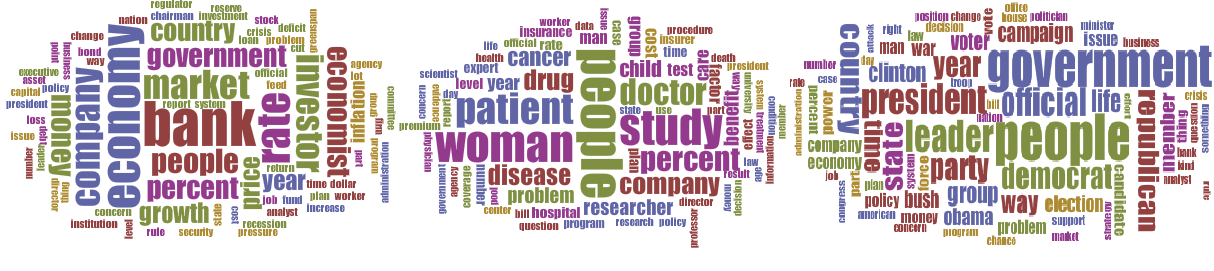
\includegraphics[width=0.70\textwidth]{../images/clouds.png}
            \caption{Key participants in the \emph{Economics}, \emph{Health} and \emph{Politics} subcorpora}
            \label{fig:clouds}
            \end{figure}

            \begin{figure}[htb!]
            \centering
            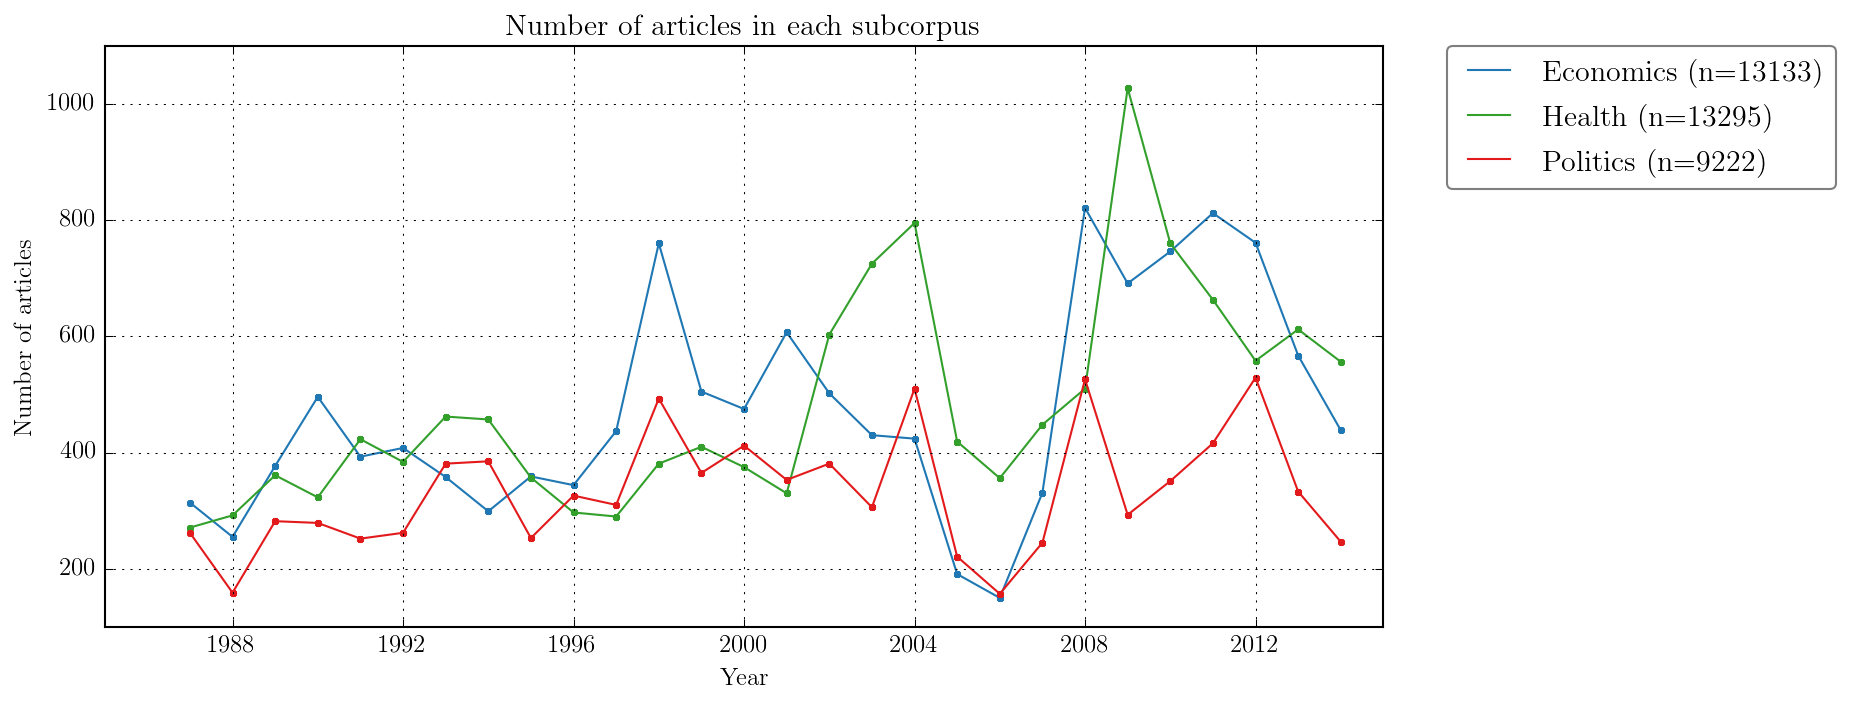
\includegraphics[width=.70\textwidth]{../images/number-of-articles-in-each-subcorpus.png}
            \caption{Number of articles in each subcorpus}
            \label{fig:article_per_subcorpus}
            \end{figure}

            \begin{figure}[htb!]
            \centering
            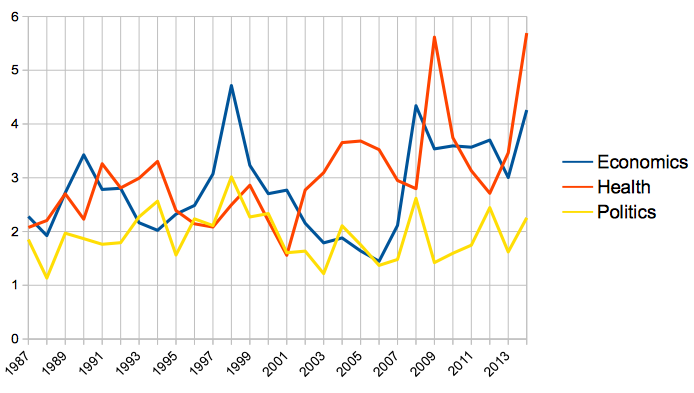
\includegraphics[width=.70\textwidth]{../images/echepol_riskwords.png}
            \caption{Risk words per total number of article topics per year}
            \label{fig:echepol_riskwords}
            \end{figure}
            %
            %Due to time constraints, we restricted the topic comparison to domains that had yielded interesting insights in the earlier interrogations. Further, we found that the smaller size of the subcorpora limited us to lexicogrammatical queries that outputted a large enough number of results for quantitative reliability. Thus, we focussed on the following three areas:

             \begin{table}[htb!]
             \centering
             \small
             \begin{tabular}{|l|l|l|}
                          \hline
                          \textbf{Economics}   & \textbf{Health}         & \textbf{Politics}     \\ \hline
                          political   & high           & political    \\ \hline
                          big         & great          & great        \\ \hline
                          economic    & low            & big          \\ \hline
                          financial   & other          & high         \\ \hline
                          great       & serious        & own          \\ \hline
                          high        & financial      & serious      \\ \hline
                          more        & potential      & new          \\ \hline
                          real        & medical        & real         \\ \hline
                          systemic    & more           & considerable \\ \hline
                          significant & significant    & more         \\ \hline
                          new         & cardiovascular & other        \\ \hline
                          little      & political      & significant  \\ \hline
                          global      & possible       & economic     \\ \hline
                          serious     & small          & financial    \\ \hline
                          other       & real           & potential    \\ \hline
                          excessive   & such           & personal     \\ \hline
                          potential   & genetic        & little       \\ \hline
                          such        & ovarian        & such         \\ \hline
                          much        & same           & public       \\ \hline
                          own         & bad            & military     \\ \hline
                          \end{tabular}
                          \caption{Most common adjectives modifying nominal risks in the topic subcorpora}
                          \label{tab:echepo_adjmod}
             \end{table}

\section{Health}

    Our topic subcorpora were much smaller than our main corpus. As a result, lexicogrammatical querying did not yield quantitatively reliable results. Accordingly, other kinds of corpus linguistic investigation, not reliant on grammatical structure, were applied. 

    First, we considered \emph{keywords}---that is, words that were unusually frequent within the health corpus when compared to the corpus as as a whole.

    Linear regression was used to determine the slope of each keyword's trajectory, and ensure that the p-value of this slope was below 0.05. Results were then sorted into two groups, based on the incline\slash decline of the slope.

    \begin{figure}[htb!]
    \centering
    \begin{minipage}{.48\textwidth}
    \centering
    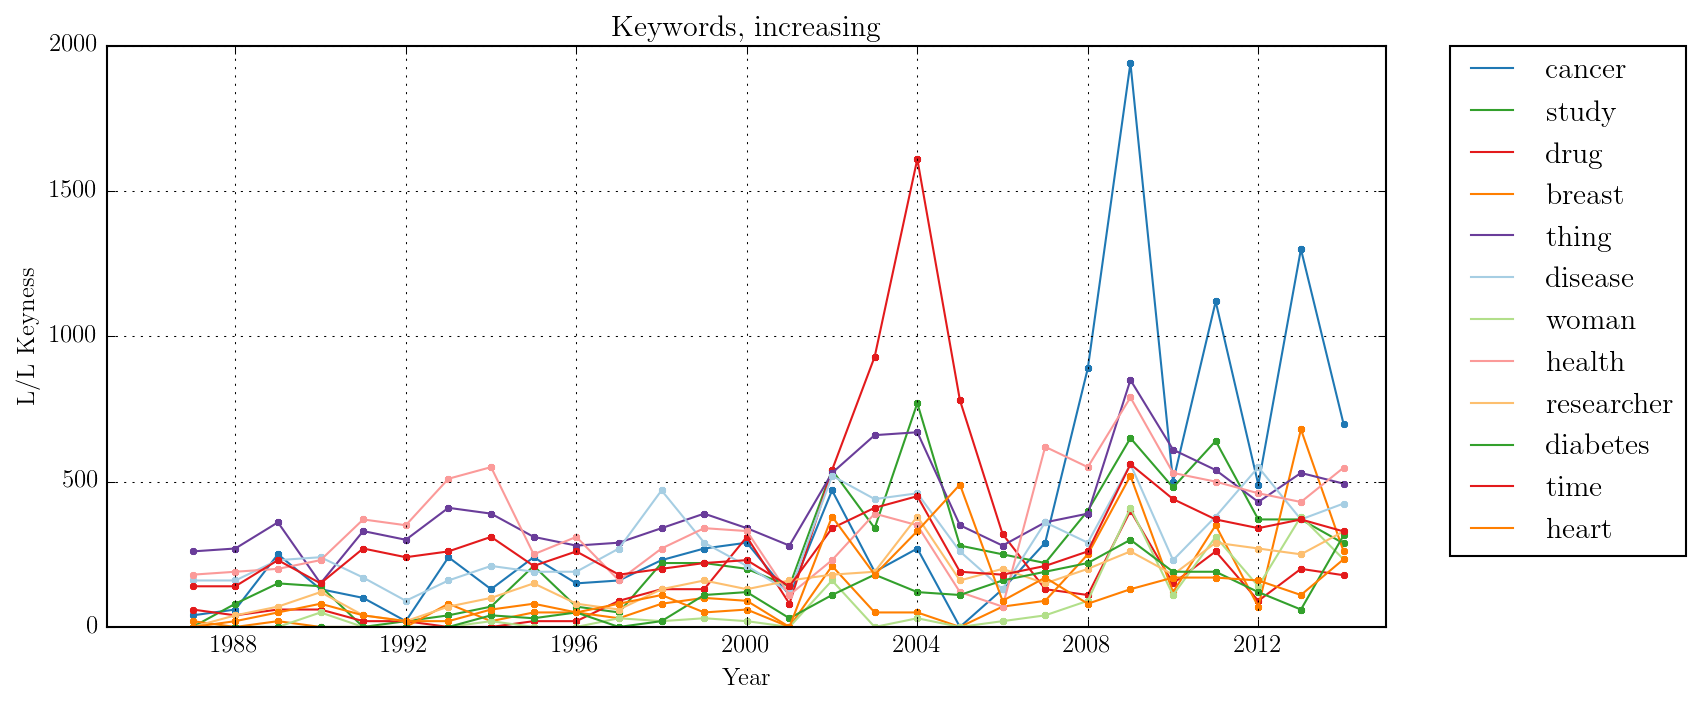
\includegraphics[width=.95\textwidth]{../images/keywords-increasing.png}
    \caption{Keywords becoming more key over time}
    \label{fig:key-inc}
    \end{minipage}%
    \begin{minipage}{.48\textwidth}
    \centering
    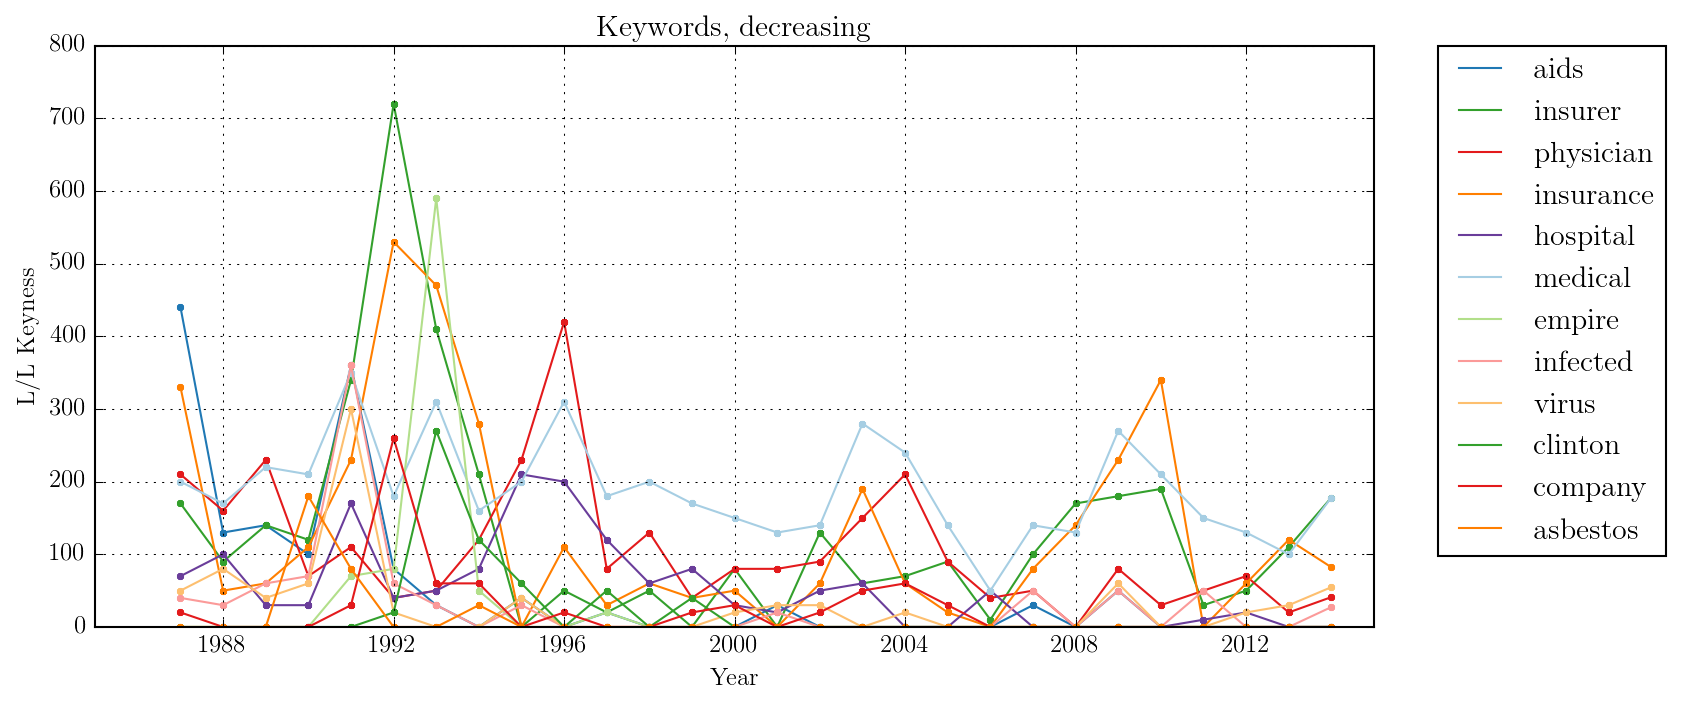
\includegraphics[width=.95\textwidth]{../images/keywords-decreasing.png}
    \caption{Keywords becoming less key over time}
    \label{fig:key-dec}
    \end{minipage}
    \end{figure}

    Next, we were interested in \emph{bigrams}---that is, words that occur beside each other multiple times within a corpus. Bigrams containing a stopword were excluded from analysis, as these results were generally common clusters of closed class words (\emph{in the}, \emph{of a}, \emph{one day}, etc.). Again, linear regression was used to group results into increasing and decreasing groups.

    \noindent
    \begin{figure}[htb!]
    \centering
    \begin{minipage}{.48\textwidth}
    \centering
    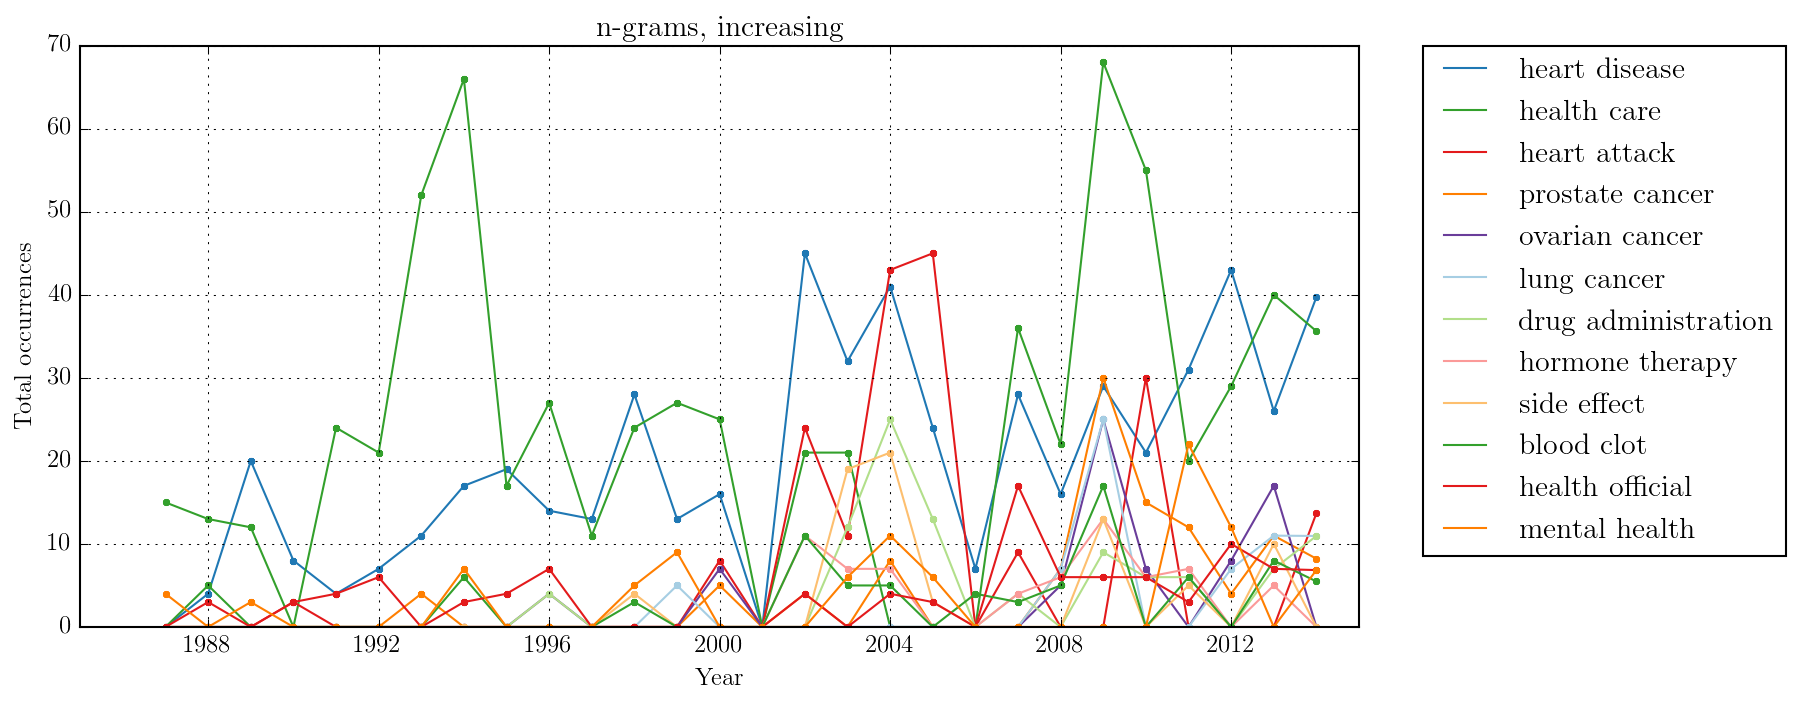
\includegraphics[width=.95\textwidth]{../images/ngrams-increasing.png}
    \caption{bi-grams becoming more frequent over time}
    \label{fig:ngram-inc}
    \end{minipage}%
    \begin{minipage}{.48\textwidth}
    \centering
    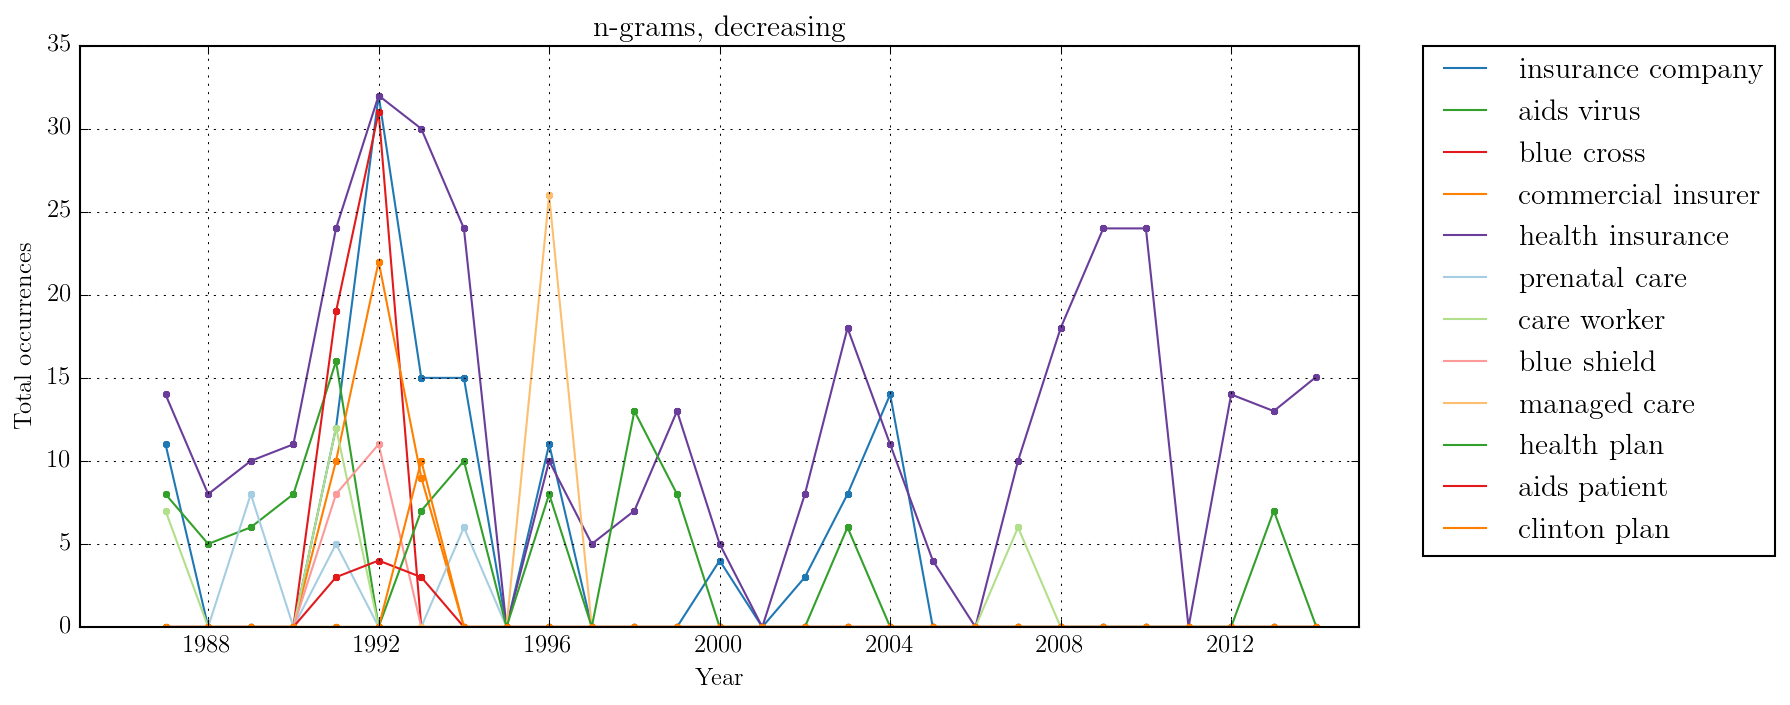
\includegraphics[width=.95\textwidth]{../images/ngrams-decreasing.png}
    \caption{bi-grams becoming less frequent over time}
    \label{fig:ngram-dec}
    \end{minipage}
    \end{figure}

We grouped these into themes, with results entered into one or more categories. Ambiguous results were often concordanced in order to determine the main context of use: \emph{athlete}, for example, could indicate the health condition (\emph{Athlete's foot}), a chain of footwear stores, or denote athletes themselves. The latter was revealed to be by far the most common context, and athlete was thus added to \emph{People, everyday}.

\subsection{Nominal groups in the health subcorpus}

The final part of our investigation of the health subcorpus looked at key nouns or nominal groups. By measuring the slope of trend lines, we could ascertain which groups were becoming more or less common.

    \noindent
    \begin{figure}[htb!]
    \centering
    \begin{minipage}{.48\textwidth}
    \centering
    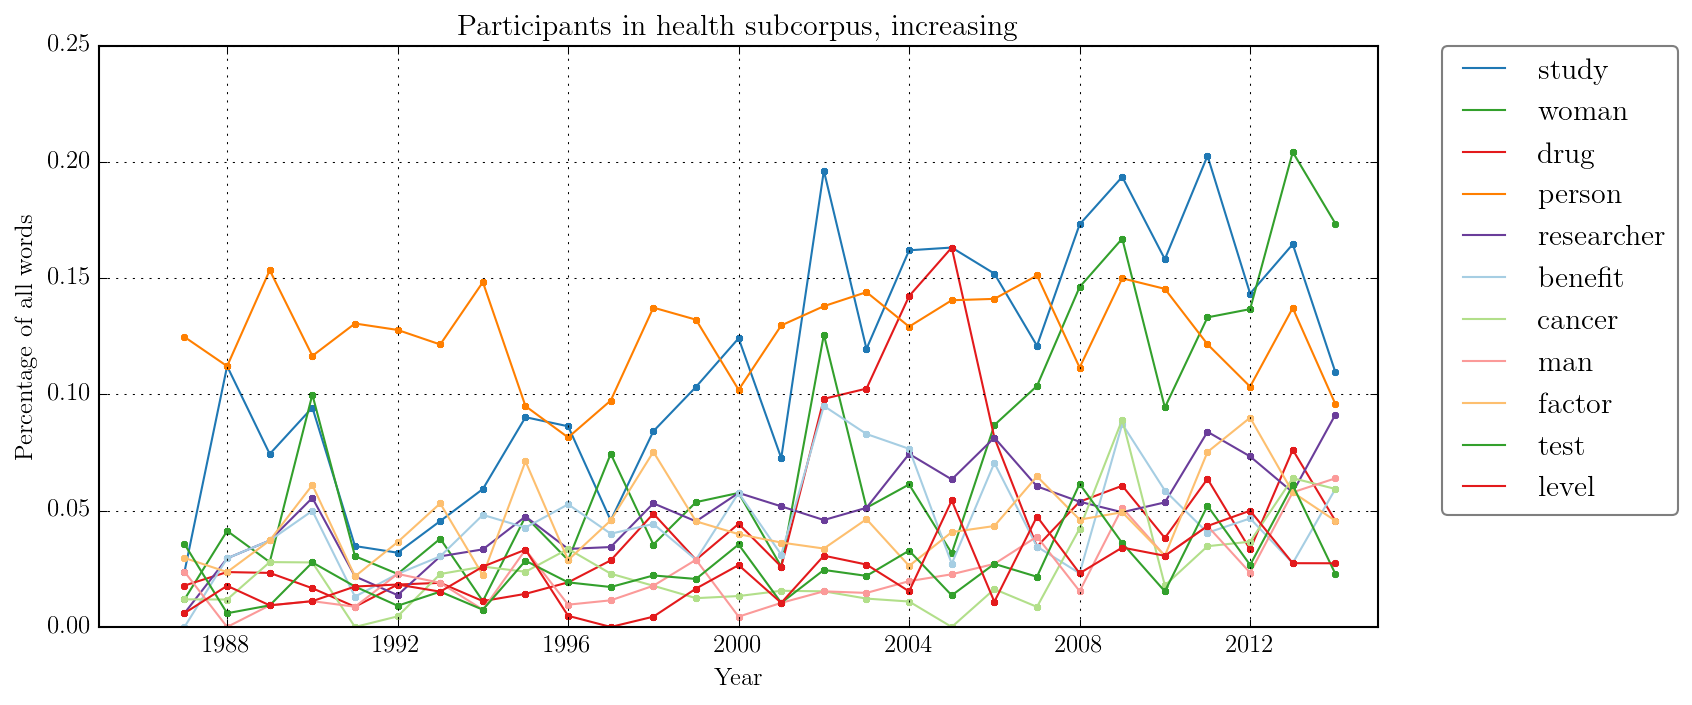
\includegraphics[width=.95\textwidth]{../images/1.png}
    \caption{Absolute frequency of nominal groups becoming more frequent over time}
    \label{fig:1}
    \end{minipage}%
    \begin{minipage}{.48\textwidth}
    \centering
    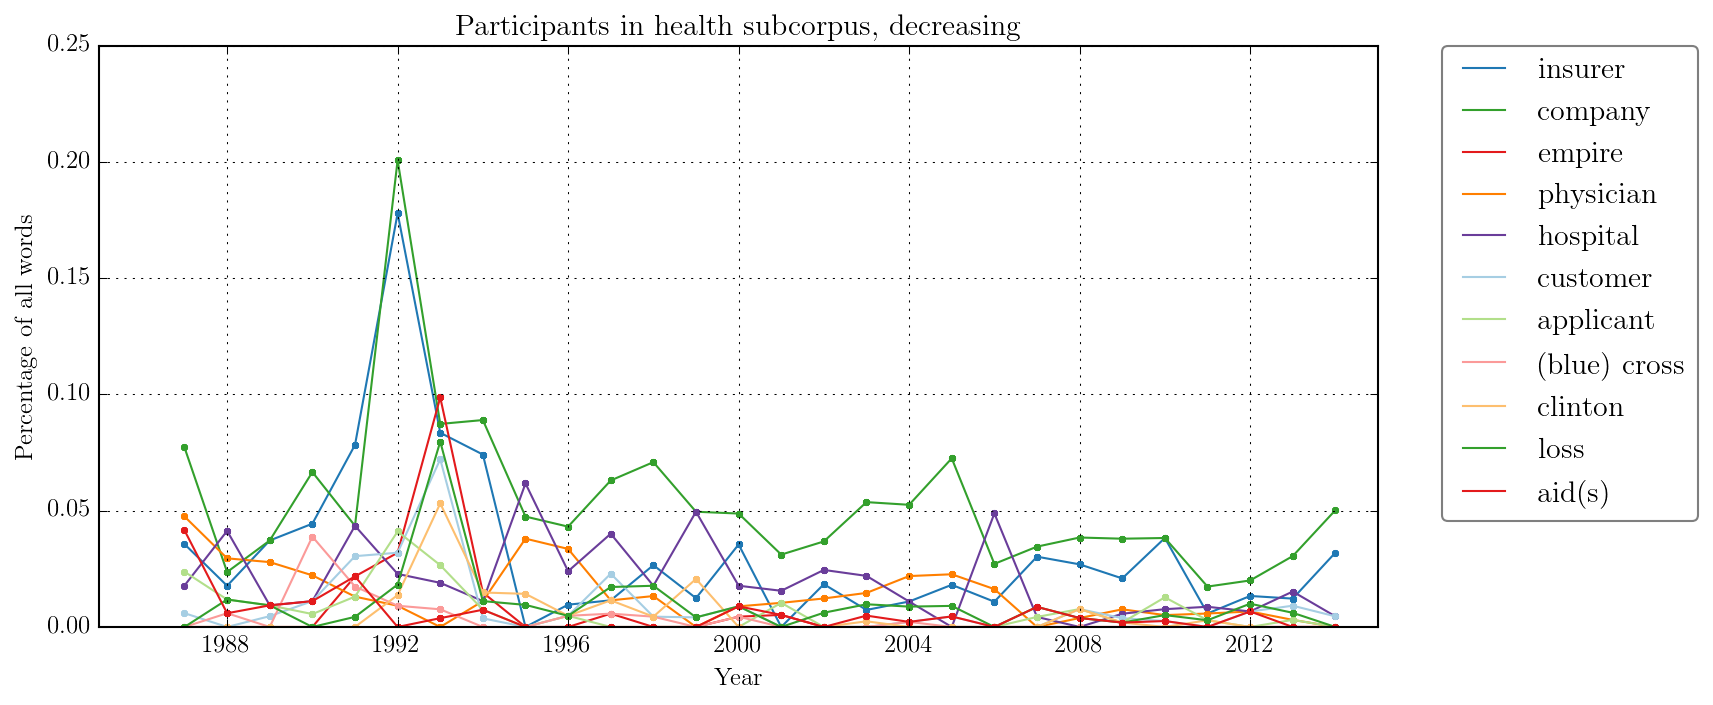
\includegraphics[width=.95\textwidth]{../images/2.png}
    \caption{Relative frequency of nominal groups becoming more frequent over time}
    \label{fig:2}
    \end{minipage}
    \end{figure}
    \noindent
    \begin{figure}[htb!]
    \centering
    \begin{minipage}{.48\textwidth}
    \centering
    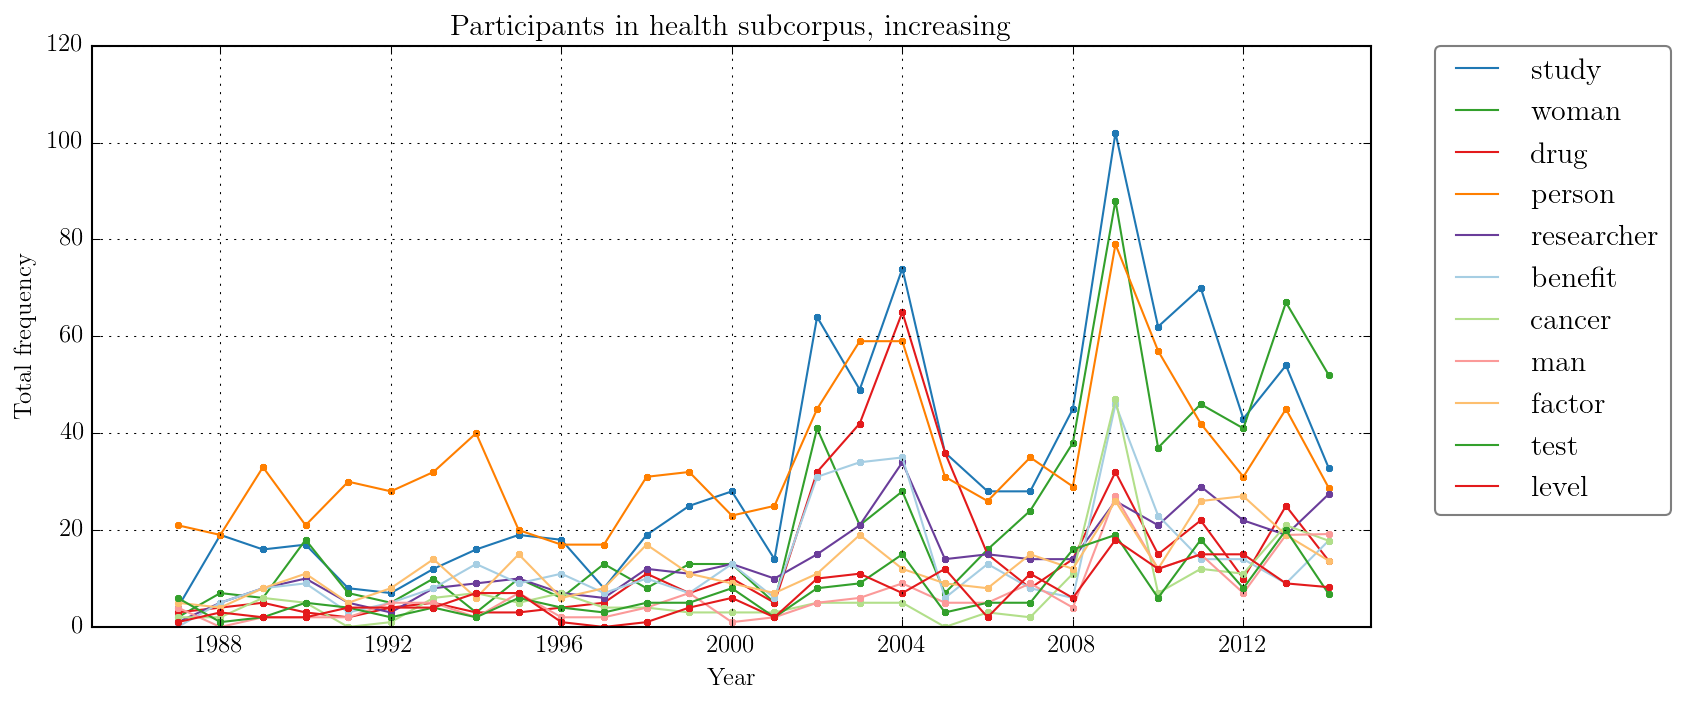
\includegraphics[width=.95\textwidth]{../images/3.png}
    \caption{Relative frequency of nominal groups becoming more frequent over time}
    \label{fig:3}
    \end{minipage}%
    \begin{minipage}{.48\textwidth}
    \centering
    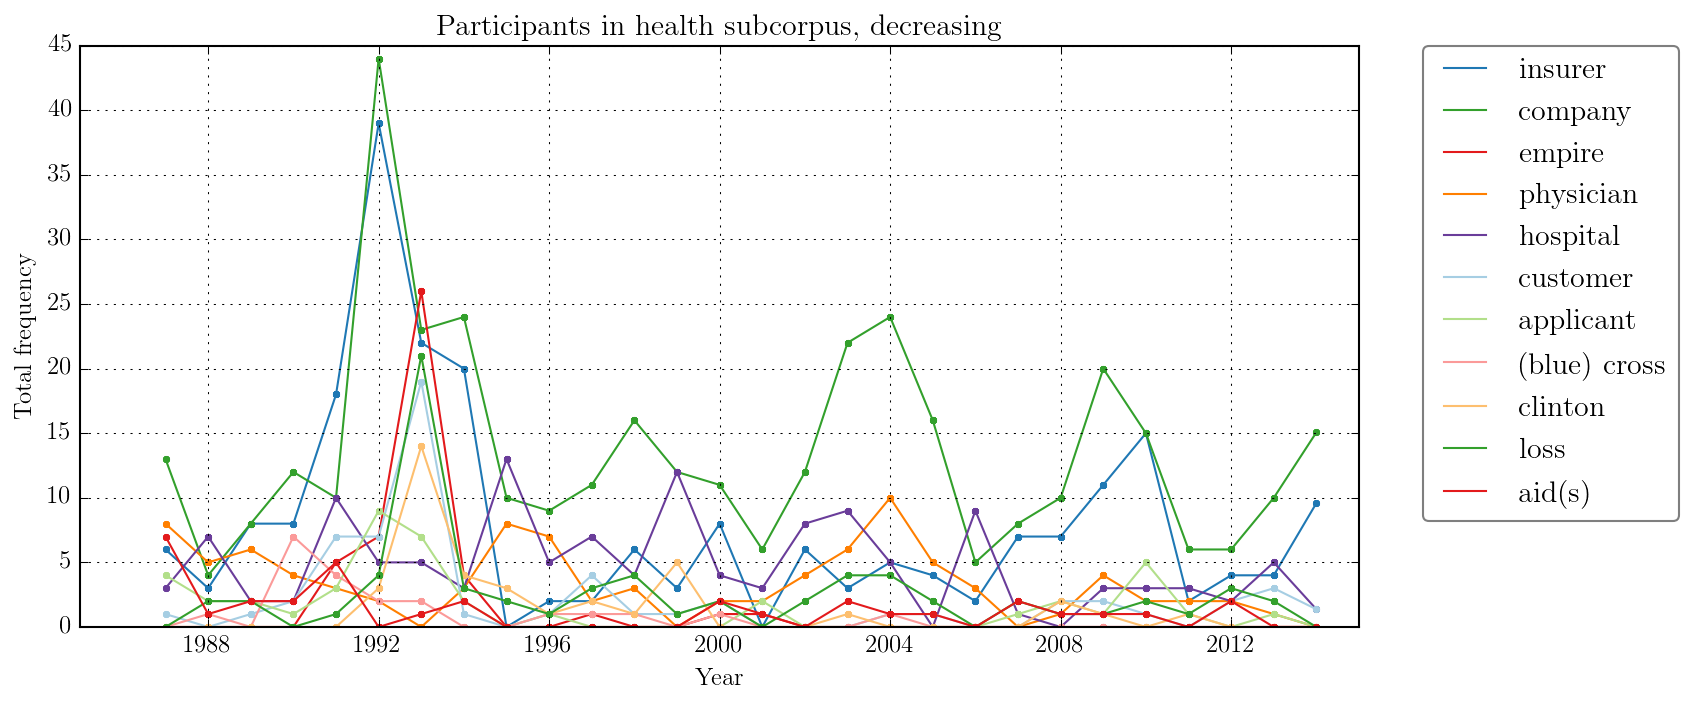
\includegraphics[width=.95\textwidth]{../images/4.png}
    \caption{Relative frequency of nominal groups becoming less frequent over time}
    \label{fig:4}
    \end{minipage}
    \end{figure}

The first major theme that emerges from this interrogation is the shift from infectious to non-infectious disease.

A second point of interest is the decline in terms related to insurance.

Though the prevalence of health insurance in mid 1990s articles was unexpected, as it corresponds with Hillary Clinton's efforts to increase health insurance coverage in the USA, unexpected was the lack of an upswing in insurance terms during the pushes for healthcare reform throughout the Obama administration.

Also apparent is an upward trend for nominal groups related to research (\emph{study, percent, research, etc.}).

This finding was of particular interest, given that the increasing contestation of academic and scientific research are core hypotheses made by Beck.

Concordancing was used to look for evidence of contestation when the nominal groups related to research were instantiated.

\section{Summary}

Broadly speaking, institutional social actors, political representatives and the like appear to have been displaced by individual human actors and components within their everyday life world.

The exception to this rule is research, which

Though further investigation into the emergence of research as a key semantic domain within risk discourse is needed, we hypothesise that it

The increasing commonality of data journalism, where journalists may conduct

Another potential factor is that the exponential increase in academic publications, as well as the increasing ease of access (via the web) has made reporting of 

This may also be a part of the increase in health risk discourse as well.

The lack of contestation points to an area in which Beck's conceptualisation of risk in late modernity may be at odds




\section{Issues in the health corpus investigation}

The first major issue was the smaller size of the corpus, which necessitated different kinds of analysis.

Within keywording and ngramming, it became clear that broader linguistic change and specific events are difficult to separate.

This, however, is where we can see the clearest examples of the link between events and language change. Interspersed throughout the keywords and n-grams are terms ranging in specificity. It is through categorisation of these varying levels that we can smooth out the 

The keywording in particular revealed a number of ambiguities. A more reliable\slash systematic method for grouping keywords would ameliorate this concern.

\section{Summary}

    The smaller size of topic subcorpora necessitated different kinds of analysis. Fortunately, such methods are well documented within corpus assisted discourse studies. Following on from these methodologies, we located particularly frequent terms, and analysed them in their context of use.

    % analysis here

    Ultimately, the ways in which a corpus can be analysed are dependent on the size of the corpus. 


%Comparing the behaviour of risk words in three smaller corpora is complicated by the lack of existing methodologies.

\afterpage{%
\begin{table}
\centering
\tiny
\begin{tabular}{|lrcl|}
\hline
1 & We know this now because                           & researchers & tested both theories , side by side , to see which \\
2 & something the public did not : Yale University     & researchers & had tentatively concluded that PPA was linked to a \\
3 & Instead ,                                          & researchers & say , young killers must be seen as extremely      \\
4 & of men with E.D. , or at risk for developing it ,  & researchers & in Italy found that the men could improve their    \\
5 & If you were an academic                            & researcher  & , you 'd have to persuade your institutional       \\
6 & Some                                               & researchers & believe hyperthymics may be at increased risk of   \\
7 & index , smoking and several other risk factors ,   & researchers & found that women on postmenopausal hormone therapy \\
8 & will have public health consequences , the         & researchers & said                                               \\
9 & Finally , and perhaps most powerfully ,            & researchers & say that a life in poverty is a life of stress     \\
10 & Office of Protection from Research Risks said the  & researchers & altered the medical records of patients , then     \\
11 & In their paper , the                               & researchers & noted that `` countries in which wine is the       \\
12 & In another study , by                              & researchers & at the University of Connecticut , leg strength    \\
13 & In an unexpected finding , the                     & researchers & reported that the women receiving goserelin also   \\
14 & that , far from protecting the heart as many       & researchers & had assumed , the therapy may have put the women   \\
15 & Now                                                & researchers & have found that elevated risk of psychiatric       \\
16 & of a New York Fire Department rescue company and a & researcher  & who is exploring the psychological bases of        \\
17 & Department of Veterans Affairs said the California & researchers & did not properly assess the safety of experimental \\
18 & Other                                              & researchers & , working with similar kinds of data , have        \\
19 & The                                                & researchers & concluded that the study '' provides the first     \\
20 & On the other hand , said Dr. Susan Czajkowski , a  & researcher  & at the National Heart , Lung and Blood Institute   \\
21 & exactly how a given AIDS patient was infected ,    & researchers & do not know exactly how much the risk of           \\
22 & In an effort to finance debts , '' the             & researchers & said , `` ordinary people are paying the ultimate  \\
23 & during the next 25 years of about 6 percent , the  & researchers & found                                              \\
24 & To obtain consent ,                                & researchers & are required to explain that the experiments are   \\
25 & slightly increasing their risks of dying earlier , & researchers & reported yesterday                                 \\
26 & Utah                                               & researchers & have videotaped 150 couples to measure the effect  \\
27 & blood cells -- became patients ' property ,        & researchers & taking them without detailed consent and explicit  \\
28 & In mapping the human genome ,                      & researchers & determined that nearly 99 percent of genetic       \\
29 & The                                                & researchers & were unable to include family history of diabetes  \\
30 & of Internal Medicine , Dr. Solomon and other       & researchers & looked at the comparative risks posed by different \\
31 & the perception of risk , said Pete Delaney , a     & researcher  & with the administration , adding that only about 9 \\
32 & The                                                & researchers & conclude that irregular sleep by itself may be a   \\
33 & Dr. Bernard H. Fox , a federal                     & researcher  & who became a pioneer in investigating the effect   \\
34 & The                                                & researchers & said it was unclear why smoking appeared to        \\
35 & The Stanford                                       & researchers & , who included Dr. Irving Weissman , a leading     \\
36 & But                                                & researchers & like Dr. Monahan and Dr. McNiel are applying       \\
37 & A study of 1,240 people by                         & researchers & at Case Western Reserve University in Cleveland    \\
38 & that of diabetes , '' said Dr. Steven G. Deeks , a & researcher  & at the University of California , San Francisco    \\
39 & In addition ,                                      & researchers & hope that the studies linking the disorder to      \\
40 & night on WNBC-TV , that Cornell University         & researchers & have found a risk of alcoholism among New York     \\
41 & , suggesting chance could play a role , but        & researchers & say the trends are credible because they are       \\
42 & The                                                & researchers & also found that patients became significantly less \\
43 & Over all ,                                         & researchers & found that calcium supplements did not lower the   \\
44 & of the power AIDS activists have mustered to push  & researchers & to do experiments that many experts deem foolish   \\
45 & The                                                & researchers & next study the extent to which medical treatment   \\
46 & was the fourth-leading risk factor for death , the & researchers & said                                               \\
47 & study 's author , Kathleen Miller , an addiction   & researcher  & at the University of Buffalo , says it suggests    \\
48 & The                                                & researchers & claim that the benefits of the research -- greater \\
49 & Some                                               & researchers & suspect genetics : Maybe thin people who develop   \\
50 & Dr. Bishop and Dr. Varmus , along with other       & researchers & , have found that the genes can cause cancer in    \\
51 & Finally ,                                          & researchers & at Tufts reported last month in The Journal of     \\
52 & The lead                                           & researcher  & , Dr. Tina V. Hartert , director of the Center for \\
53 & harmful cholesterol in the blood , even when the   & researchers & accounted for other risk factors for high          \\
54 & on cases stemming from the Sept. 11 attacks ,      & researchers & found that the more deeply therapists were         \\
55 & The                                                & researchers & did find an increased risk of other , less common  \\
56 & The inquiry in Ms. Wan 's case found that          & researchers & had adequately explained the risks to her and that \\
57 & For example , she said ,                           & researchers & are experimenting with fast-growing carp that      \\
58 & than 23,000 Greek men and women ages 20 to 86 ,    & researchers & found that napping at least three times a week for \\
59 & precision afforded by simple computing devices ,   & researchers & say , promise to deliver new insights on risk      \\
60 & only two categories of risk , minimal and great ,  & researchers & were often discouraged from doing research         \\
61 & the clear advantage of moderate drinking , the     & researchers & presented their findings with strong caveats       \\
62 & As the genes become better understood ,            & researchers & expect to find ways to block them if they become   \\
63 & adolescents followed over a period of nine years , & researchers & at the New York Psychiatric Institute found that   \\
64 & Health , for example , said that 100 psychiatric   & researchers & gathered in a room would all probably agree that   \\
65 & smoking might have damaged the fathers ' sperm ,   & researchers & said yesterday                                     \\
66 & with 20 percent of the control group , the         & researchers & found                                              \\
67 & The                                                & researchers & found that for each four-inch increase in height   \\
68 & between height and cancer may help guide           & researchers & to study hormones and growth factors that          \\
69 & Why do                                             & researchers & and willing patients test the boundaries of        \\
70 & 's disease as those who have never smoked ,        & researchers & say , and several small studies have indicated     \\
71 & But                                                & researchers & said they had never seen this before , either in   \\
72 & In 2012 , British                                  & researchers & , by combining results from clinical trials that   \\
73 & After adjusting for various health factors , the   & researchers & found that for each increase of 10 micrograms per  \\
74 & The F.D.A. has asked                               & researchers & at Columbia to reclassify the cases of self-harm   \\
75 & The                                                & researchers & said this was troubling , given recent studies     \\
76 &  A large team of                                    & researchers & , led by V. Wendy Setiawan , an assistant          \\
77 &  and violated Federal regulations because the       & researchers & had not informed patients of the risks             \\
78 &  Yet                                                & researchers & also concluded the risk of stroke was the same as  \\
79 &  In 2002 ,                                          & researchers & halted the largest clinical trial ever conducted   \\
80 &  , and while they might not be surprising to        & researchers & , they were intended to inform the public as well  \\
81 &  Many                                               & researchers & said anger-prone people could reduce the risk of   \\
82 &  Using preserved blood samples of pregnant women ,  & researchers & have found that low vitamin D levels are           \\
83 &  And so now                                         & researchers & have been working on new strategies : Developing   \\
84 &  This month , Danish                                & researchers & reported on a 15-year study of 12,000 nurses       \\
85 &  She said                                           & researchers & thought older medicine was riskier because the     \\
86 &  Last Sunday ,                                      & researchers & released data that showed that outdoor air         \\
87 &  But when the company and the                       & researcher  & are one and the same , he said , that check is     \\
88 &  Huntington 's disease and cystic fibrosis , and    & researchers & say tests identifying those at high risk of heart  \\
89 &  may increase with a father 's advancing age ,      & researchers & reported yesterday                                 \\
90 &  Denise Juliano-Bult , a                            & researcher  & at the National Institute of Mental Health , said  \\
91 &  those who gain fat around the hips and thighs ,    & researchers & say                                                \\
92 &  in the British Medical Journal in August ,         & researchers & in Argentina showed that women who were given      \\
93 &  Next ,                                             & researchers & said , they want to do a large study like one      \\
94 &  The                                                & researchers & noted that the drinks contain high levels of       \\
95 &  The                                                & researchers & offered some other examples of how the risks       \\
96 &  Some other                                         & researchers & questioned the findings , and most agreed that the \\
97 &  For purposes of comparison , the                   & researchers & also examined inherited variations in 13 genes     \\
98 &  And the flaws are compounded , the                 & researchers & said , when journalists do n't report the context  \\
99 &  A few years ago , Mercedes Carnethon , a diabetes  & researcher  & at the Feinberg School of Medicine at Northwestern \\
100 &  As with beta carotene ,                            & researchers & were shocked                                       \\
\hline
\end{tabular}
\caption{100 random instances of \emph{researcher} in the health subcorpus}
\label{tab:research}
\end{table}
\clearpage
}